\documentclass[journal,12pt,twocolumn]{IEEEtran}

\usepackage{setspace}
\usepackage{gensymb}
\singlespacing
\usepackage[cmex10]{amsmath}

\usepackage{amsthm}

\usepackage{mathrsfs}
\usepackage{txfonts}
\usepackage{stfloats}
\usepackage{bm}
\usepackage{cite}
\usepackage{cases}
\usepackage{subfig}

\usepackage{longtable}
\usepackage{multirow}

\usepackage{enumitem}
\usepackage{mathtools}
\usepackage{steinmetz}
\usepackage{tikz}
\usepackage{circuitikz}
\usepackage{verbatim}
\usepackage{tfrupee}
\usepackage[breaklinks=true]{hyperref}
\usepackage{graphicx}
\usepackage{tkz-euclide}

\usetikzlibrary{calc,math}
\usepackage{listings}
    \usepackage{color}                                            %%
    \usepackage{array}                                            %%
    \usepackage{longtable}                                        %%
    \usepackage{calc}                                             %%
    \usepackage{multirow}                                         %%
    \usepackage{hhline}                                           %%
    \usepackage{ifthen}                                           %%
    \usepackage{lscape}     
\usepackage{multicol}
\usepackage{chngcntr}

\DeclareMathOperator*{\Res}{Res}

\renewcommand\thesection{\arabic{section}}
\renewcommand\thesubsection{\thesection.\arabic{subsection}}
\renewcommand\thesubsubsection{\thesubsection.\arabic{subsubsection}}

\renewcommand\thesectiondis{\arabic{section}}
\renewcommand\thesubsectiondis{\thesectiondis.\arabic{subsection}}
\renewcommand\thesubsubsectiondis{\thesubsectiondis.\arabic{subsubsection}}


\hyphenation{op-tical net-works semi-conduc-tor}
\def\inputGnumericTable{}                                 %%

\lstset{
%language=C,
frame=single, 
breaklines=true,
columns=fullflexible
}
\begin{document}


\newtheorem{theorem}{Theorem}[section]
\newtheorem{problem}{Problem}
\newtheorem{proposition}{Proposition}[section]
\newtheorem{lemma}{Lemma}[section]
\newtheorem{corollary}[theorem]{Corollary}
\newtheorem{example}{Example}[section]
\newtheorem{definition}[problem]{Definition}

\newcommand{\BEQA}{\begin{eqnarray}}
        \newcommand{\EEQA}{\end{eqnarray}}
\newcommand{\define}{\stackrel{\triangle}{=}}
\bibliographystyle{IEEEtran}
\raggedbottom
\setlength{\parindent}{0pt}
\providecommand{\mbf}{\mathbf}
\providecommand{\pr}[1]{\ensuremath{\Pr\left(#1\right)}}
\providecommand{\qfunc}[1]{\ensuremath{Q\left(#1\right)}}
\providecommand{\sbrak}[1]{\ensuremath{{}\left[#1\right]}}
\providecommand{\lsbrak}[1]{\ensuremath{{}\left[#1\right.}}
\providecommand{\rsbrak}[1]{\ensuremath{{}\left.#1\right]}}
\providecommand{\brak}[1]{\ensuremath{\left(#1\right)}}
\providecommand{\lbrak}[1]{\ensuremath{\left(#1\right.}}
\providecommand{\rbrak}[1]{\ensuremath{\left.#1\right)}}
\providecommand{\cbrak}[1]{\ensuremath{\left\{#1\right\}}}
\providecommand{\lcbrak}[1]{\ensuremath{\left\{#1\right.}}
\providecommand{\rcbrak}[1]{\ensuremath{\left.#1\right\}}}
\theoremstyle{remark}
\newtheorem{rem}{Remark}
\newcommand{\sgn}{\mathop{\mathrm{sgn}}}
\providecommand{\abs}[1]{\left\vert#1\right\vert}
\providecommand{\res}[1]{\Res\displaylimits_{#1}}
\providecommand{\norm}[1]{\left\lVert#1\right\rVert}
%\providecommand{\norm}[1]{\lVert#1\rVert}
\providecommand{\mtx}[1]{\mathbf{#1}}
\providecommand{\mean}[1]{E\left[ #1 \right]}
\providecommand{\fourier}{\overset{\mathcal{F}}{ \rightleftharpoons}}
%\providecommand{\hilbert}{\overset{\mathcal{H}}{ \rightleftharpoons}}
\providecommand{\system}{\overset{\mathcal{H}}{ \longleftrightarrow}}
%\newcommand{\solution}[2]{\textbf{Solution:}{#1}}
\newcommand{\solution}{\noindent \textbf{Solution: }}
\newcommand{\cosec}{\,\text{cosec}\,}
\providecommand{\dec}[2]{\ensuremath{\overset{#1}{\underset{#2}{\gtrless}}}}
\newcommand{\myvec}[1]{\ensuremath{\begin{pmatrix}#1\end{pmatrix}}}
\newcommand{\mydet}[1]{\ensuremath{\begin{vmatrix}#1\end{vmatrix}}}
\numberwithin{equation}{subsection}

\makeatletter
\@addtoreset{figure}{problem}
\makeatother
\let\StandardTheFigure\thefigure
\let\vec\mathbf

\renewcommand{\thefigure}{\theproblem}

\def\putbox#1#2#3{\makebox[0in][l]{\makebox[#1][l]{}\raisebox{\baselineskip}[0in][0in]{\raisebox{#2}[0in][0in]{#3}}}}
\def\rightbox#1{\makebox[0in][r]{#1}}
\def\centbox#1{\makebox[0in]{#1}}
\def\topbox#1{\raisebox{-\baselineskip}[0in][0in]{#1}}
\def\midbox#1{\raisebox{-0.5\baselineskip}[0in][0in]{#1}}
\vspace{3cm}
\title{Assignment 2}
\author{V. L. Narasimha Reddy - EE18BTECH11046}
\maketitle
\newpage
\bigskip
\renewcommand{\thefigure}{\theenumi}
\renewcommand{\thetable}{\theenumi}
Download all python codes from
\begin{lstlisting}
https://github.com/narasimha-123/EE4013/tree/main/Assignment-2/codes
\end{lstlisting}
%
and latex-tikz codes from
%
\begin{lstlisting}
https://github.com/narasimha-123/EE4013/tree/main/Assignment-2/figs
\end{lstlisting}
\section{Problem}
Check whether three points
\[
    A =
    \begin{pmatrix}
        x_{1}  \\
        x_{2}  \\
        \vdots \\
        x_{n}
    \end{pmatrix},
    B =
    \begin{pmatrix}
        y_{1}  \\
        y_{2}  \\
        \vdots \\
        y_{n}
    \end{pmatrix},
    C =
    \begin{pmatrix}
        z_{1}  \\
        z_{2}  \\
        \vdots \\
        z_{n}
    \end{pmatrix}
\]
are collinear or not.

\section{Solution}

We can say that three points are collinear if there exists a $\lambda$
such that it satisfies the condition that is
\begin{equation}
    \overrightarrow{AB} = \lambda\overrightarrow{AC}
\end{equation}
because then we can say that the direction ratios of
three vectors A,B,C are proportional which implies
that the three points A, B and C are collinear.
i.e., if they are of form
\[
    \begin{pmatrix}
        x_{1}-y_{1} \\
        x_{2}-y_{2} \\
        \vdots      \\
        x_{n}-y_{n}
    \end{pmatrix}
    =
    \lambda \begin{pmatrix}
        x_{1}-z_{1} \\
        x_{2}-z_{2} \\
        \vdots      \\
        x_{n}-z_{n}
    \end{pmatrix}
\]

This method to check whether points are collinear can
be extended to "m" points.
\\
\newline
let $A_{1},A_{2},A_{3},...,A_{m}$ be the m points
\\
\newline
The idea is same, First we take three points of the
m points and check if the direction ratios of
three vectors are proportional. If they are proportional
that implies that the three points are collinear.
\\
So, We check the proportionality of direction ratios
for different combination of 3 points each time.
If in all the cases the direction ratios of
three vectors are proportional, then we can say that
all points are collinear. i.e., they satisfy the
condition
\\
\begin{equation}
    \overrightarrow{A_{i}A_{i+1}} = \lambda\overrightarrow{A_{i}A_{i+2}}
\end{equation}
$\forall$ i $\epsilon$ ${0,1,2,...m-2}$

The code to check collinearity is found in
\begin{lstlisting}
    ./codes/ee18btech11046.c
\end{lstlisting}

\section{Example}
Check whether points
\[
    A =
    \begin{pmatrix}
        1 \\
        2 \\
        7
    \end{pmatrix},
    B =
    \begin{pmatrix}
        2 \\
        6 \\
        3
    \end{pmatrix},
    C =
    \begin{pmatrix}
        3  \\
        10 \\
        -1
    \end{pmatrix}
\]
are collinear or not.

\section{Solution for example}
We can say that the points are collinear if the three points A, B
, C satisfy the above condition
\begin{equation}
    \overrightarrow{AB} = \lambda\overrightarrow{AC}
\end{equation}

Now,
\begin{equation}
    \overrightarrow{AB} =
    \begin{pmatrix}
        -1 \\
        -4 \\
        4
    \end{pmatrix}
\end{equation}
and
\begin{equation}
    \overrightarrow{AC} =
    \begin{pmatrix}
        -2 \\
        -8 \\
        8
    \end{pmatrix}
\end{equation}
We can see that $\overrightarrow{AC}$ can be written as
\begin{equation}
    \overrightarrow{AC} =2
    \begin{pmatrix}
        -1 \\
        -4 \\
        4
    \end{pmatrix}
\end{equation}
\begin{equation}
    \overrightarrow{AC} = 2\overrightarrow{AB}
\end{equation}
which is of form
\begin{equation}
    \overrightarrow{AB} = \lambda\overrightarrow{AC}
\end{equation}
where $\lambda$ is equal to $\frac{1}{2}$.

Since the direction ratios of the given points A, B, C are proportional
, We can say that the given points are Collinear.

\section{Verification}

We plotted the given three points in 3d-plotting using python.
The points in 3d-plane are as shown below.

The code to generate the python plot for the three is
found in
\begin{lstlisting}
    ./codes/ee18btech11046.py
\end{lstlisting}

\begin{figure}[!ht]
    \centering
    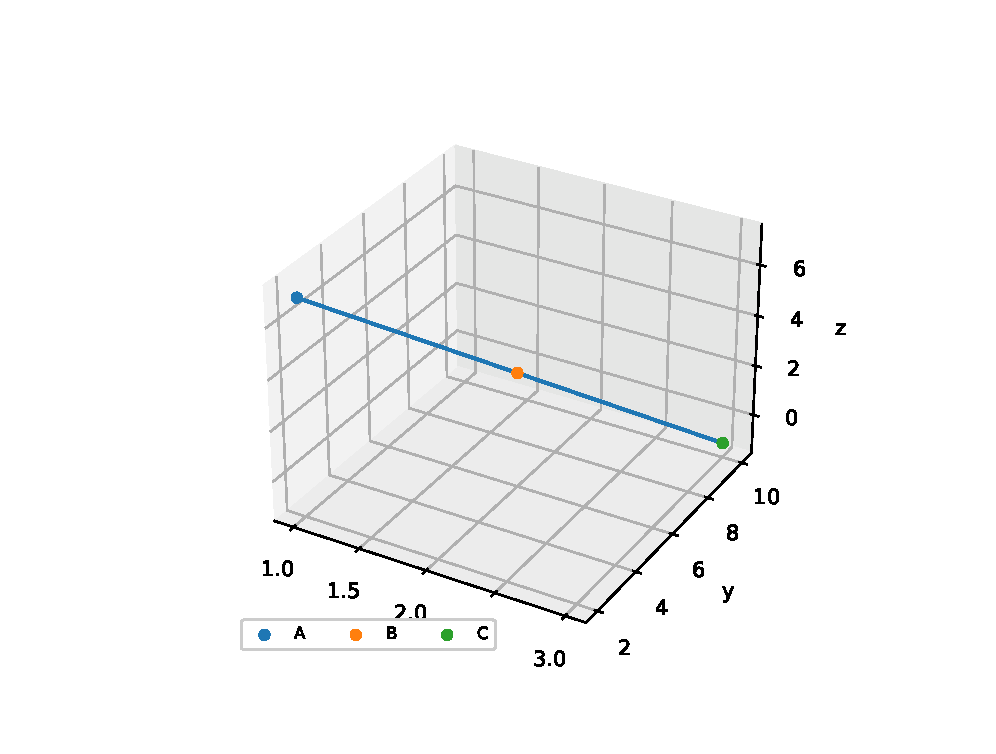
\includegraphics[width=\columnwidth]{./figs/ee18btech11046.eps}
    \caption{3D plot of given points}
    \label{fig:3Dplot}
\end{figure}

From the figure we can see that the three given points are on same line.
Therefore the given points are collinear.


\end{document}